\documentclass[10pt]{beamer}
\usetheme{metropolis}
\usepackage{booktabs}
\usepackage{tabularx}
\usepackage{calc}
\usepackage{tikz}

\usetikzlibrary{shapes.geometric, positioning, decorations.pathreplacing, shadows, arrows.meta, calc}

% Setup for faculty images
\newlength{\imageheight}
\setlength{\imageheight}{3.5cm}

% Define CSUF brand colors
\definecolor{titanblue}{HTML}{00244E}
\definecolor{mediumblue}{HTML}{0F3F8C}
\definecolor{skyblue}{HTML}{EBFBFF}
\definecolor{titanorange}{HTML}{FF7900}
\definecolor{titangray}{HTML}{F5F5F5}
\definecolor{titantext}{HTML}{222222}
\definecolor{warningred}{HTML}{D7263D} % Added missing color definition

% Customize metropolis theme colors
\setbeamercolor{normal text}{fg=titantext, bg=white}
\setbeamercolor{alerted text}{fg=titanorange}
\setbeamercolor{example text}{fg=mediumblue}

% Title page colors
\setbeamercolor{title}{fg=titanblue, bg=white}
\setbeamercolor{subtitle}{fg=mediumblue, bg=white}
\setbeamercolor{institute}{fg=titanorange, bg=white}
\setbeamercolor{date}{fg=titanblue, bg=white}

% Frame title colors
\setbeamercolor{frametitle}{fg=white, bg=titanblue}
\setbeamercolor{framesubtitle}{fg=mediumblue, bg=white}

% Block environment colors
\setbeamercolor{block title}{fg=white, bg=titanblue}
\setbeamercolor{block body}{fg=titantext, bg=skyblue!10}

% Item colors
\setbeamercolor{itemize item}{fg=titanorange}
\setbeamercolor{itemize subitem}{fg=mediumblue}
\setbeamercolor{itemize subsubitem}{fg=titanblue}

% Footer and header colors
\setbeamercolor{footer}{fg=titantext}
\setbeamercolor{header}{fg=titanblue}

% Customize fonts
\setbeamerfont{title}{size=\Large, series=\bfseries}
\setbeamerfont{frametitle}{size=\large, series=\bfseries}

% Simple title page template
\defbeamertemplate*{title page}{customized}[1][]
{
\vspace{1cm}
 {\usebeamerfont{title}\usebeamercolor[fg]{title}\inserttitle\par}
\vspace{0.5cm}
 {\usebeamerfont{subtitle}\usebeamercolor[fg]{subtitle}\insertsubtitle\par}
\vspace{0.5cm}
 {\usebeamerfont{date}\usebeamercolor[fg]{date}\insertdate\par}
\vfill
 {\insertinstitute\par}
}

% Add progress bar
\makeatletter
\setbeamertemplate{headline}{%
\begin{beamercolorbox}[wd=\paperwidth,ht=0.4cm,dp=0cm]{titanblue}%
\begin{tikzpicture}
\pgfmathsetmacro{\progress}{\insertframenumber/\inserttotalframenumber}
\fill[titanorange] (0,0) rectangle (\progress*\paperwidth,0.4cm);
\end{tikzpicture}%
\end{beamercolorbox}%
}
\makeatother

\begin{document}

\title{Understanding Politics and Public Policy}
\subtitle{Foundations and Core Concepts \\ POSC 315: Introduction to Public Policy \\ Lecture 8-3: Decision Making (Part 3 of 3)}
\date{David P. Adams, Ph.D.}
\institute{California State University, Fullerton}

\maketitle

\begin{frame}{Decision-Making Models Overview}
\begin{itemize}
  \item \textbf{Rational Choice:} Idealized model based on full information and optimization.
  \item \textbf{Bounded Rationality:} Limited information and satisficing behavior.
  \item \textbf{Incrementalism:} Policy change through small, conservative steps.
  \item \textbf{Groupthink:} When group harmony overrides critical thinking.
  \item \textbf{Garbage Can Model:} Organized anarchy; decisions emerge from timing.
\end{itemize}
\end{frame}

\begin{frame}{Groupthink: Key Symptoms}
\begin{block}{Definition}
Prioritizing group cohesion and unanimity over critical analysis.
\end{block}
\vspace{0.5cm}
\textbf{Common Symptoms:}
\begin{itemize}
  \item Illusion of invulnerability
  \item Collective rationalization
  \item Suppression of dissent
  \item Self-censorship
\end{itemize}
\end{frame}

\begin{frame}{Groupthink: Prevention Strategies}
\begin{block}{Strategies to Avoid Groupthink}
\begin{itemize}
  \item Encourage open dialogue and dissent
  \item Assign a devil's advocate role
  \item Use anonymous feedback mechanisms
  \item Break into smaller groups for discussion
  \item Rotate leadership roles
\end{itemize}
\end{block}
\begin{block}{Goal}
To ensure diverse perspectives are considered and critical thinking is maintained.
\end{block}
\end{frame}   

\begin{frame}{Groupthink: Example}
\begin{block}{Example: Bay of Pigs Invasion}
In 1961, President Kennedy's advisors:
\begin{itemize}
  \item Overvalued consensus and ignored dissenting opinions.
  \item Failed to critically evaluate the risks of the invasion.
  \item Resulted in a poorly planned operation that ended in failure.
\end{itemize}
\end{block}
\end{frame} 

\begin{frame}{Garbage Can Model of Decision-Making}
\begin{block}{Core Idea}
Problems, solutions, participants, and choice opportunities float independently and only occasionally align.
\end{block}
\begin{itemize}
  \item Developed by Cohen, March, and Olsen (1972)
  \item Reflects high-uncertainty, loosely coupled organizations
\end{itemize}
\end{frame}

\begin{frame}{Four Streams in the Garbage Can Model}
\begin{itemize}
  \item \textbf{Choices} looking for problems
  \item \textbf{Issues} looking for decision venues
  \item \textbf{Solutions} looking for problems
  \item \textbf{Participants} looking for something to do
\end{itemize}
\textbf{When these converge by chance:} a decision is made.
\end{frame}

% --- helper macro for smooth S-curves ---
% #1 = source node, #2 = target coord, #3/#4 = y-offsets for control points
\newcommand{\smoothstream}[4]{%
  \draw[streamarrow]
    (#1.east)
      .. controls ($(#1.east)+(0.90, #3)$) and ($(#2)+(-1.30, #4)$)
      .. (#2);
}

\begin{frame}{Garbage Can Model: Streams Visualization}
\centering
\vspace{-0.2cm}
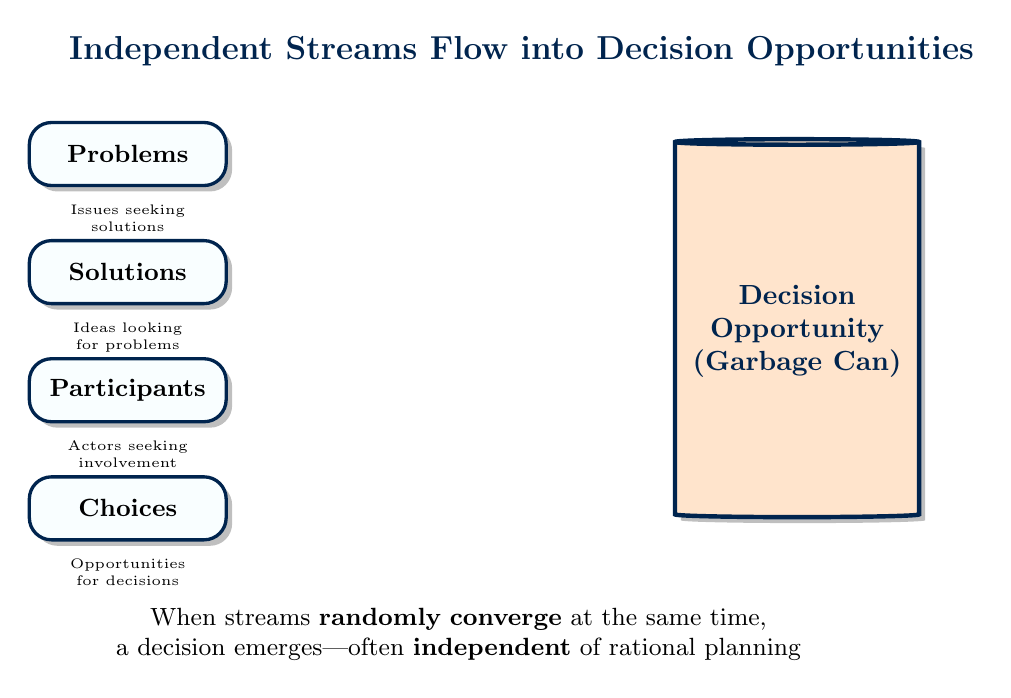
\begin{tikzpicture}[
  stream/.style={
    draw=titanblue, very thick, rounded corners=8pt,
    minimum width=2.5cm, minimum height=0.8cm,
    font=\small\bfseries, fill=skyblue!30, drop shadow
  },
  % prettier arrows
  streamarrow/.style={
    -{Latex[length=3.2mm,width=2.6mm]},  % crisp tip
    ultra thick, draw=titanorange!90,
    line cap=round, line join=round,
    shorten <=2pt, shorten >=2pt
  },
  label/.style={font=\tiny, align=center, text width=2.3cm}
]

% Title
\node[font=\bfseries\large, titanblue] at (5,3.8)
  {Independent Streams Flow into Decision Opportunities};

% Streams (left)
\node[stream] (problems)    at (0, 2.50) {Problems};
\node[label,  below=0.1cm of problems] {Issues seeking\\solutions};

\node[stream] (solutions)   at (0, 1.00) {Solutions};
\node[label,  below=0.1cm of solutions] {Ideas looking\\for problems};

\node[stream] (participants)at (0,-0.50) {Participants};
\node[label,  below=0.1cm of participants] {Actors seeking\\involvement};

\node[stream] (choices)     at (0,-2.00) {Choices};
\node[label,  below=0.1cm of choices] {Opportunities\\for decisions};

% Garbage can
\node[
  draw=titanblue, ultra thick, cylinder, shape border rotate=90,
  minimum height=4.8cm, minimum width=3.1cm,
  fill=titanorange!20, drop shadow, aspect=0.30
] (can) at (8.5,0.25) {};

\node[font=\bfseries, titanblue, align=center] at (8.5,0.25)
  {Decision\\Opportunity\\(Garbage Can)};

% --- landing pads on the LEFT edge of the can (clean targets) ---
\path let \p1 = (can.west) in
  coordinate (canTop)  at (\x1, { \y1 + 1.45})
  coordinate (canHi)   at (\x1, { \y1 + 0.55})
  coordinate (canLo)   at (\x1, { \y1 - 0.65})
  coordinate (canBot)  at (\x1, { \y1 - 1.55});

% Streams → Can (tweak the control offsets to taste)
\smoothstream{problems}{canTop}{ 0.35}{ 0.70}
\smoothstream{solutions}{canHi}{  0.10}{ 0.40}
\smoothstream{participants}{canLo}{-0.20}{-0.30}
\smoothstream{choices}{canBot}{  -0.10}{-0.60}

% Footer
\node[font=\small, align=center, text width=10cm] at (4.2,-3.6) {
  When streams \textbf{randomly converge} at the same time,\\
  a decision emerges—often \textbf{independent} of rational planning
};
\end{tikzpicture}
\end{frame}

\begin{frame}{Garbage Can Model: Example}
\begin{block}{Example: University Budgeting}
Imagine a university where:
\begin{itemize}
  \item \textbf{Problems:} Departments need more funding.
  \item \textbf{Solutions:} New fundraising strategies.
  \item \textbf{Participants:} Faculty, administrators, and students.
  \item \textbf{Choices:} Budget meetings scheduled at random times.
  \item \textbf{Outcome:} A decision is made when a fundraising idea aligns with a budget meeting, even if not all problems are addressed.
\end{itemize}
\end{block}
\end{frame}

\begin{frame}{Comparison Table: Decision-Making Models}
\begin{tabularx}{\textwidth}{l X X X}
\toprule
\textbf{Model} & \textbf{Information} & \textbf{Process} & \textbf{Outcome} \\
\midrule
Rational Choice & Complete & Optimization & Best solution \\
Bounded Rationality & Limited & Satisficing & Good enough \\
Incrementalism & Limited & Small steps & Gradual change \\
Groupthink & Filtered & Conformity & Poor decisions \\
Garbage Can & Random & Stream convergence & Unpredictable \\
\bottomrule
\end{tabularx}
\end{frame}

\begin{frame}{Decision-Making Toolkit}
\begin{block}{\textbf{Rational Analysis} -- When info is good}
Use when you have reliable data, time, and a clear problem. 
\end{block}

\begin{block}{\textbf{Satisficing} -- When time is short}
Use when decisions must be made quickly with limited info. 
\end{block}

\begin{block}{\textbf{Incrementalism} -- When risk is high}
Use when radical change is risky or politically infeasible. 
\end{block}

\begin{block}{\textbf{Groupthink Prevention} -- Build in dissent}
Use when teams are at risk of overvaluing harmony. 
\end{block}

\begin{block}{\textbf{Opportunity Recognition} -- Be ready when streams align}
Use when solutions, problems, and decision windows collide. 
\end{block}
\end{frame}

\begin{frame}{Final Thought}
\begin{quote}
\textbf{``The best decision-makers aren't those who follow one model perfectly, but those who know which model to use when.''}
\end{quote}
\end{frame}

\end{document}
